A phasor model of the system shown in Fig. \ref{fig:Feeder2} is modeled and simulated  in MATLAB\textsuperscript{\textregistered} Simulink\textsuperscript{\textregistered} using the Simscape Power Systems\textsuperscript{TM} toolbox for validating the algorithm. Fig. \ref{fig:without_vvc} shows the per-unit feeder bus voltages for 86,400 seconds (24 hours) without implementing the control algorithm. The legends V1, V2, V3, V4, V5, V6, V7, V8 and V9 in the figure represent the per-unit (PU) voltages of buses B20010P, B20020P, B20030P, B20040P, B20050P, B20060P, B20070P, B20080P, and B20090P respectively. As it can be seen in the figure, the bus voltages drop below the 0.95 PU limit when the algorithm is not activated.

\begin{figure}[!h]
\centering
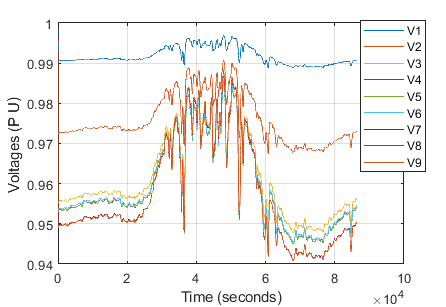
\includegraphics[width=\linewidth]{figs/CVC/Without_VVC.png}
\caption{Voltage Profile without Coordinated Voltage Control}
\label{fig:without_vvc}
\end{figure}

Fig. \ref{fig:with_cvc} presents the voltage profiles of all the nodes in the system with the coordinated voltage control activated. To show the effectiveness of the proposed algorithm the voltage bounds were set between 0.97 PU and 1.01 PU. It can be seen in the figure that the algorithm is capable of maintaining the voltages within the bounds by coordinating the DG inverters and capacitor banks available in the system. Fig. \ref{fig:DG_Q} shows the reactive power supplied by the DGs during the simulation. Fig \ref{fig:cap_bank} shows the switching states of capacitor banks Cap.B20040P, Cap.B20030P and Cap.B20070P. The capacitor bank Cap.B20060P is not used to regulate voltage because it is defined as always on in the system specification. The switching status 1 means that the capacitor bank is connected and the switching status 0 means that the capacitor bank is disconnected. It can be seen from the figures that the coordinated voltage control algorithm was able to maintain the system voltage status within the bounds mostly by using the DG inverters. It required two switching operations from the cap bank Cap.B20070P in addition to the DG inverters capability to maintain system voltage within 0.97 PU and 1.01 PU. It should be noted that during the full 24-hour simulation the on load tap changing transformer situated between buses B20010P and 20000P was not required to control the system voltage. From Fig. \ref{fig:with_cvc} it can also be inferred that the algorithm responds rapidly to voltage violations. In the actual simulation, the algorithm always performed the required calculations under a second.

\begin{figure}[!h]
\centering
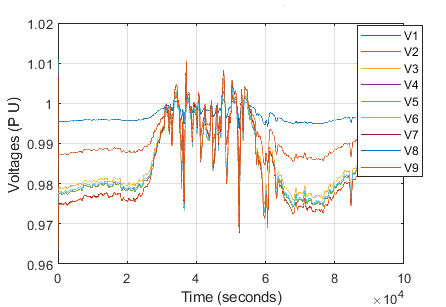
\includegraphics[width=\linewidth]{figs/CVC/With_VVC.png}
\caption{Voltage profile with coordinated voltage control}
\label{fig:with_cvc}
\end{figure}

\begin{figure}[!h]
\centering
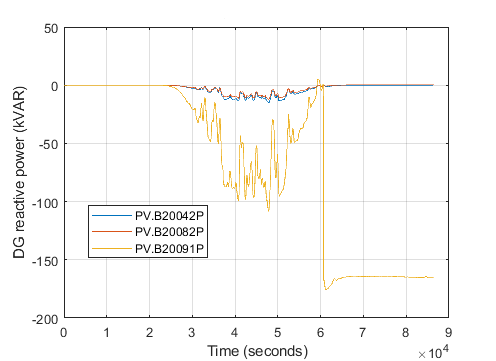
\includegraphics[width=\linewidth]{figs/CVC/DG_Q.png}
\caption{Reactive power supplied by DGs}
\label{fig:DG_Q}
\end{figure}

\begin{figure}[!h]
\centering
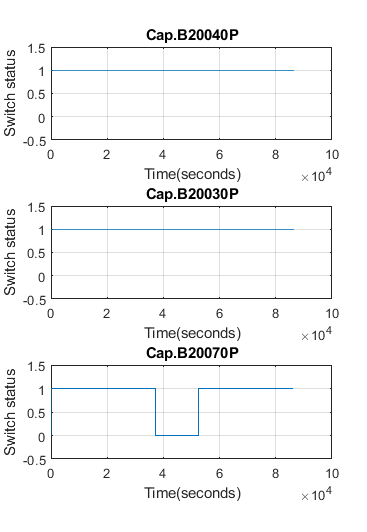
\includegraphics[width=0.8\linewidth]{figs/CVC/CAP_BANK.png}
\caption{Capacitor bank switching states}
\label{fig:cap_bank}
\end{figure}
